% \documentclass[tikz,border=10pt]{standalone}
% \usepackage{tikz}
% \usetikzlibrary{angles,quotes,calc}

% \begin{document}
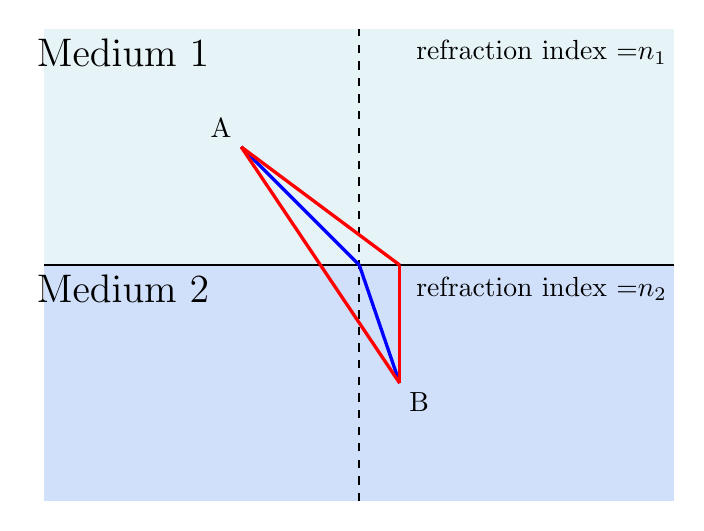
\begin{tikzpicture}
    % Define colors
    \definecolor{medium1}{RGB}{173,216,230}  % Light blue for air
    \definecolor{medium2}{RGB}{100,149,237}  % Darker blue for water/glass

    % Draw the two media
    \fill[medium1, opacity=0.3] (-4,0) rectangle (4,3);
    \fill[medium2, opacity=0.3] (-4,-3) rectangle (4,0);

    % Draw the interface line
    \draw[thick] (-4,0) -- (4,0);

    % Draw the normal line (dashed)
    \draw[dashed, thick] (0,-3) -- (0,3);

    % Define angles
    \def\incidentangle{90}
    \def\refractedangle{20}

    % Calculate ray endpoints and helper coordinates
    \coordinate (A) at ({-1.5*sin(\incidentangle)}, 1.5);  % Incident ray start
    \coordinate (O) at (0,0);                           % Point of incidence
    \coordinate (B) at ({1.5*sin(\refractedangle)}, -1.5);  % Refracted ray end
    \coordinate (N1) at (0,2);                          % Normal point above
    \coordinate (N2) at (0,-2);                         % Normal point below

    % Draw incident ray
    \draw[-, very thick, blue] (A) -- (O);

    % Draw refracted ray  
    \draw[-, very thick, blue] (O) -- (B);

    % Straight line
    \draw[-, very thick, red] (A) -- (B);

    % Long path
    \draw[-, very thick, red] (A) -- ({1.5*sin(\refractedangle)},0);
    \draw[-, very thick, red] (B) -- ({1.5*sin(\refractedangle)},0);

    % Add medium labels
    \node[above] at (-3,2.4) {\Large Medium 1};
    \node[below] at (-3,0) {\Large Medium 2};
    \node[right] at (0.6,2.7) {refraction index =$n_1$};
    \node[right] at (0.6,-0.3) {refraction index =$n_2$};

    % Add point labels
    \node[above left] at (A) {A};
    \node[below right] at (B) {B};

\end{tikzpicture}
% \end{document}
